%\documentclass[dvipdfmx]{beamer}
\documentclass[dvipdfmx,final,t,10pt]{beamer}
\usepackage[orientation=portrait,size=a4,scale=1.4]{beamerposter}%縦 : orientation=portrait, 横 : orientation=landscape
\usepackage{here, amsmath, latexsym, amssymb, bm, ascmac, mathtools, multicol, tcolorbox}
\usepackage{listings}
%\usepackage{luatexja}
%\usepackage{luatexja-otf}
%\usepackage[match]{luatexja-fontspec}
%\usepackage[]{luatexja-preset}

%\AtBeginDvi{\special{pdf:mapfile ptex-ipa.map}}

\renewcommand{\kanjifamilydefault}{\gtdefault}
\usepackage[deluxe, expert]{otf}
\usepackage{minijs}  %min10

\lstset{
    frame=single,
    basicstyle={\ttfamily\footnotesize},
}

%カラーテーマの選択(省略可)
%\usecolortheme{orchid}
\usetheme{zurichposter}
%フォントテーマの選択(省略可)
\usefonttheme{professionalfonts}
%フレーム内のテーマの選択(省略可)
\useinnertheme{circles}

%ナビゲーションバー非表示
\setbeamertemplate{navigation symbols}{}
%既定をゴシック体に
\renewcommand{\kanjifamilydefault}{\gtdefault}
%itemize
%\setbeamertemplate{itemize item}{\small\raise0.5pt\hbox{$\bullet$}}
%\setbeamertemplate{itemize subitem}{\tiny\raise1.5pt\hbox{$\blacktriangleright$}}
%\setbeamertemplate{itemize subsubitem}{\tiny\raise1.5pt\hbox{$\bigstar$}}
% color
%\newcommand{\red}[1]{\textcolor{red}{#1}}
%\newcommand{\green}[1]{\textcolor{green!40!black}{#1}}
%\newcommand{\blue}[1]{\textcolor{blue!80!black}{#1}}
%head
%\setbeamertemplate{headline}{
%    \begin{center}
%        \structure{
%            \vskip3ex
%            \rule{0.98\linewidth}{4mm}
%            \vskip3ex
%            \usebeamercolor{title in headline}{\textbf{\LARGE{\inserttitle}}\\[2.5ex]}
%            \usebeamercolor{author in headline}{\large{\insertauthor}\\[1.2ex]}
%            \usebeamercolor{institute in headline}{\large{\insertinstitute}}
%            \vskip3ex
%            \rule{0.98\linewidth}{4mm}
%        }
%    \end{center}
%}


\setbeamerfont{block title}{size=\Large}
\setbeamerfont{block body}{size=\large}

\setbeamertemplate{itemize/enumerate body begin}{\large}
\setbeamertemplate{itemize/enumerate subbody begin}{\large}
\setbeamertemplate{itemize/enumerate subsubbody begin}{\large}

%\setbeamersize{text margin left = 2.5ex, text margin right = 1.2ex}
\setbeamersize{text margin left = 2.5ex, text margin right = 2.5ex}
%\addtobeamertemplate{block begin}{\ }{}
%\setbeamercolor{block body}{bg=gray}

\title{組込みシステム向けFRP言語の\\実行モデルの並列化}
\author{櫻井義孝・渡部卓雄}
\institute{東京工業大学}


\begin{document}

\begin{frame}[fragile]
    \vskip -2.5ex
    \begin{block}{概要}
        \vskip 1ex
        \begin{itemize}
            \item 本研究の目的は小規模組込みシステム向けFRP言語の応答性向上である.
            \item 既存の小規模組込みシステム向けFRP言語であるEmfrpはシングルスレッドで動作する.
                \begin{itemize}
                    \item マルチスレッドが使用可能な環境では計算資源を十分に活用できない.
                \end{itemize}
            \item 本研究では応答性向上のために静的スケジューリングを用いてEmfrpを並列化することを提案する.
        \end{itemize}
        \vskip -2.5ex
    \end{block}

    \begin{block}{Emfrp \small{[Sawada2016]}}
        \begin{columns}
            \begin{column}{0.4\textwidth}
                \vskip -1.15ex
                小規模組込みシステム向けFRP言語
                \lstinputlisting{./code/FanController.xfrp}
                \begin{center}
                    \vskip -3ex
                    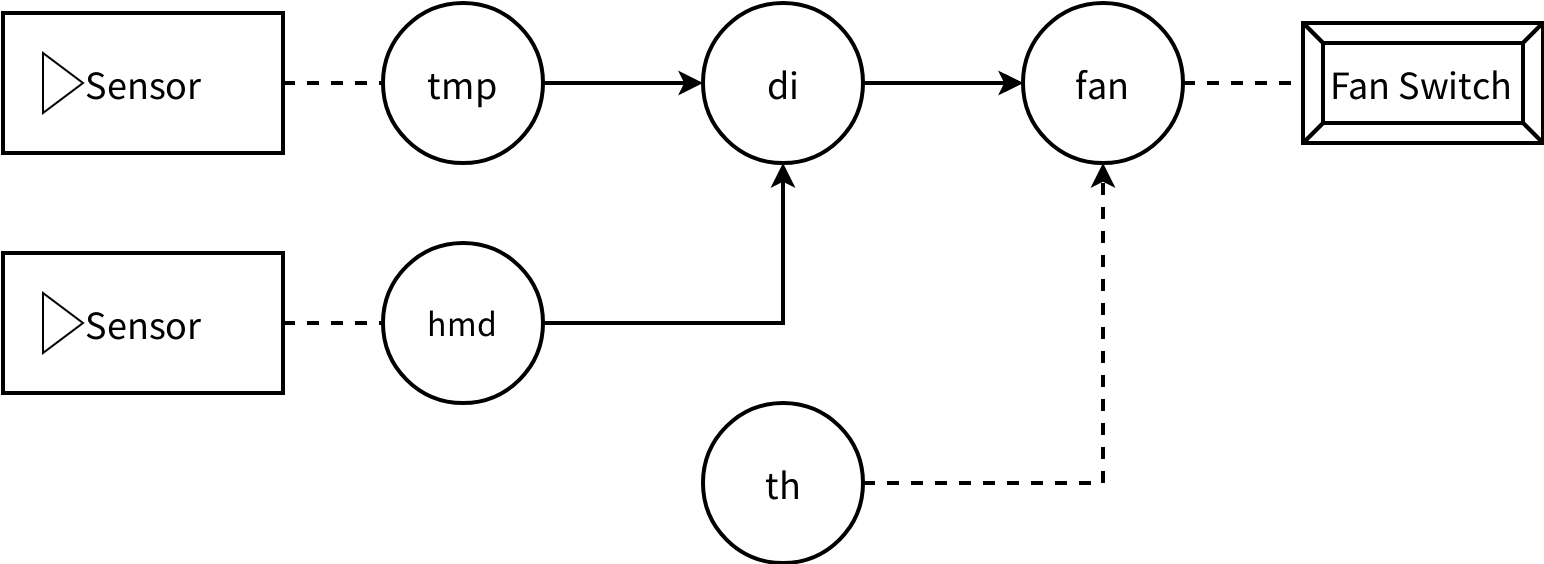
\includegraphics[scale=0.3]{./image/FanController.png}
                \end{center}
            \end{column}
            \begin{column}{0.55\textwidth}
                \vskip -0.4cm
                \begin{itemize}
                    \item Emfrpのプログラムは,時変値をノードとし依存関係を辺とした有向非巡回グラフ(DAG)を構成する.
                    \item 現在のEmfrpの処理系ではノードの更新は逐次的に行われる.左に挙げた例の場合,DAGをトポロジカルソートしたtmp$\rightarrow$hmd$\rightarrow$di$\rightarrow$th$\rightarrow$fanの順に更新が行われる.この更新(サイクル)を繰り返すことでリアクティブな動作を実現している.
                    \item 1サイクルにかかる時間がシステムの応答性を決める.本研究では,マルチコアシステムでの応答性向上を目的とした並列化方式を提案する.実行環境として汎用的なOSだけでなく,OSのない環境やFreeRTOS程度の小規模RTOSを考える.
                    \item 本研究の想定環境にはOSによるスケジューラによる適切なスケジューリングが期待できない環境も含まれている.そのため,実行モデルを並列化する際に実行モデルはOSのスケジューラに依存しないで動作する必要がある.
                    \item 本研究では,各サイクルの計算時間を短縮し,可能であれば応答時間を予測できるような静的スケジューリング方式を提案する.
                \end{itemize}
            \end{column}
        \end{columns}
    \end{block}

    \begin{block}{並列化アルゴリズム}
        \vskip -0.3cm
        \begin{columns}
            \begin{column}{0.6\textwidth}
                \begin{enumerate}
                    \item 各ノードからsinkノードへの最長距離を計算する.
                    \begin{itemize}
                        \item sinkノードは出次数が0のノード(右図では赤いノード)
                    \end{itemize}
                    \item 同じ距離にあるノードを並列に更新する.
                        \begin{itemize}
                            \item OSのスケジューラを利用できない環境ではそれぞれのノードをどのプロセッサが更新するかを指定する必要がある.
                            \item これは各スレッドがなるべく同じ数になるように割り当てる.
                                \begin{itemize}
                                    \item 下の表のsinkノードへの距離0のノード$3,5,7,8,9$を2スレッドで処理するならば$3,5$をスレッド1が$7,8,9$をスレッド2が更新.
                                \end{itemize}
                        \end{itemize}
                \end{enumerate}
                \vskip-0.3cm
                \begin{table}[h]
                    \begin{tabular}{|c|c|c|c|}
                        \hline
                        出力ノードまでの距離 & 2   & 1     & 0                                                    \\ \hline
                        同時に処理するノード & 0,4 & 1,2,6 & \begin{tabular}[c]{@{}l@{}}3,5,\\ 7,8,9\end{tabular} \\ \hline
                    \end{tabular}
                \end{table}
            \end{column}
            \begin{column}{0.3\textwidth}
                \begin{center}
                    \vskip-0.1cm
                    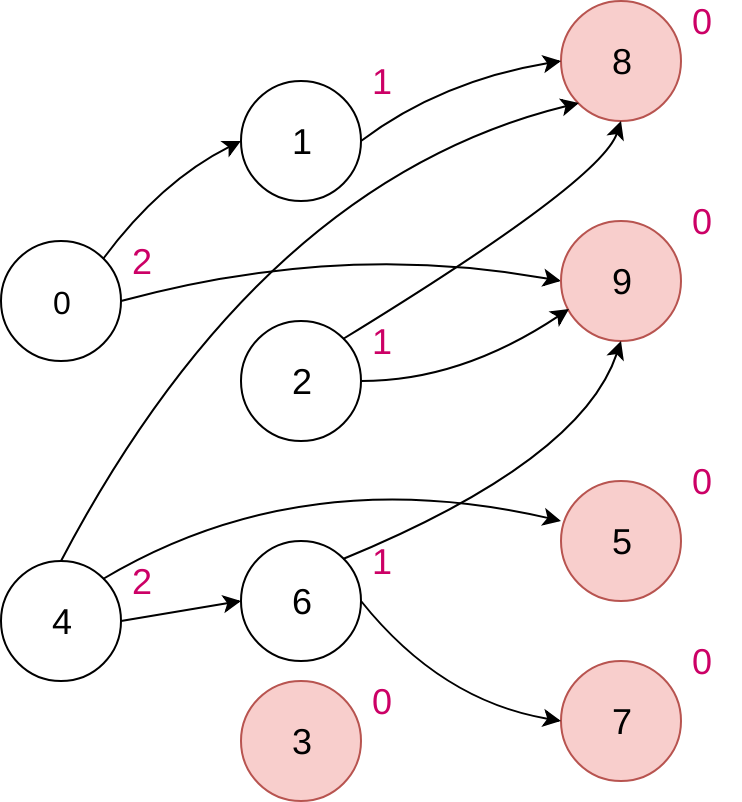
\includegraphics[scale=0.18]{image/RandomGraph.png}
                \end{center}
            \end{column}
        \end{columns}
        \vskip-.7cm
    \end{block}

    \begin{block}{実験}
        \vskip 0.2cm
            提案する並列化アルゴリズムの性能を評価するために,XFRP-Core上で提案する実行モデルとEmfrpの実行モデルを実装し,一定サイクルにかかる時間を測定した.
            実験環境には,Intel Core i7-975,RAM12GB上のUbuntu12.04を使用した.
            本実験では並列化にはPthreadを使用した.
            実験対象のアプリケーションとして,LifeGameと熱拡散シュミレータをXFRP上で実装した.
            実験では100000サイクルにかかる時間を10回計測し,その平均を扱った.
            実験結果は以下の表のようになった.
        \begin{columns}
            \begin{column}{0.5\textwidth}
                \begin{table}
                    \begin{tabular}{|l|c|r|r|} \hline
                        アプリケーション & Emfrp & XFRP-Core(2) & XFRP-Core(4) \\ \hline
                        LifeGame & 203.61(sec) & 108.04(sec) & 64.05(sec) \\ \hline
                    \end{tabular}
                \end{table}
            \end{column}
            \begin{column}{0.4\textwidth}
                %\vskip -3.2cm
                左はLifeGameを30000ループするのにかかった時間であり,右はノードに30000ナノ秒のビジーウェイトを挟んで100ループしたときにかかった時間である.
                左では4スレッド使用したにも関わらず30\%程度しか時間が削減できていない.
                一方で,ノードの実行時間が大きくると右のように4スレッドで実行時間が27\%になった.
            \end{column}
        \end{columns}
    \end{block}
\end{frame}
\end{document}
